\documentclass{article}
\usepackage{graphicx} % Required for inserting images
\usepackage[margin=1in]{geometry}
\usepackage{wrapfig}
\usepackage{subcaption}
\usepackage{hyperref}

\title{CISC856 A2}
\author{Teodor Ilie}
\date{\today}

\begin{document}

\maketitle

\textit{Note: All code is my own, with some ideas taken from \href{https://www.geeksforgeeks.org/sarsa-reinforcement-learning/}{GeeksForGeeks} for the basic Sarsa implementation.}

\section{Windy Gridworld}
First I compare performance and hyperparameter choices for the regular windy gridworld environment as defined by Sutton and Barto.
\subsection{Comparison and Hyperparameter Choice for Sarsa, Q-Learning}
For Sarsa, good hyperparameter options are $\alpha = 0.5, \epsilon = 0.1$. These are commonly used, including in the Sutton and Barto textbook on pg. 130. The same values work for Q-Learning, although other values are also commonly chosen, such as $\alpha \in [0.1, 0.5]$ and $\epsilon \in [0.1, 0.3]$. t

These $\alpha$ values ensure fast but stable learning, and the $\epsilon$ values are a good balance of exploration and exploitation. Figure \ref{fig:hyperparam} shows a graphical comparison of other value combinations. As can be seen, other values work similarly or worse.

Note that due to the stochastic nature of the processes, there is some variability in the results. However, Q-Learning outperforms Sarsa consistently for standard parameter choices, as Sarsa completes 170 episodes in around 8000 time steps, while Q-Learning completes the same 170 episodes in around 7000 time steps.

\begin{figure}[h!]
  \centering
  \begin{subfigure}{0.45\textwidth} 
    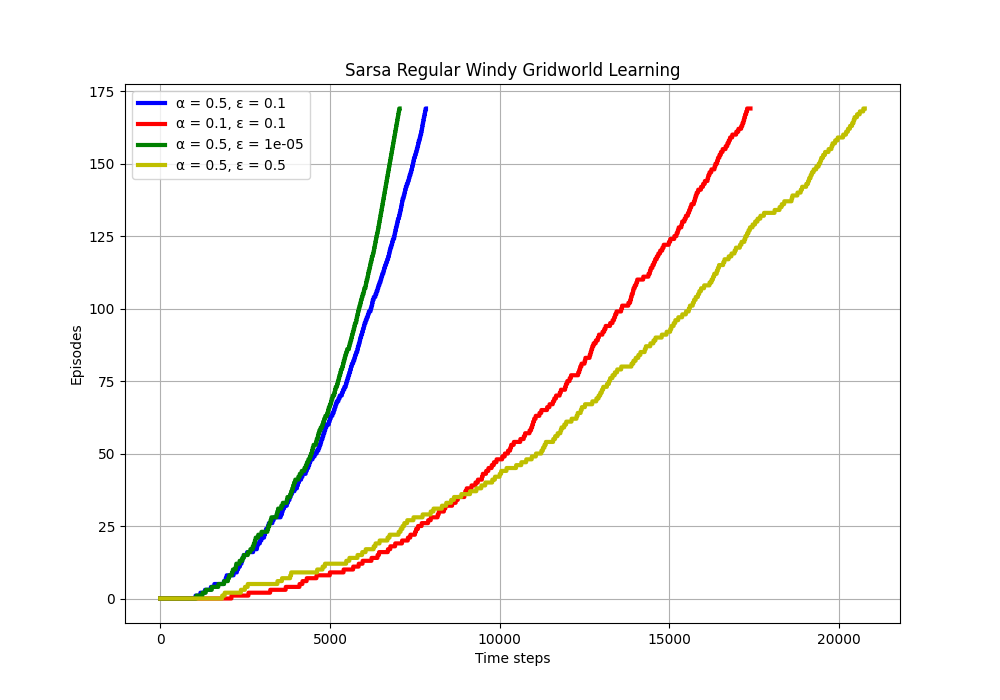
\includegraphics[width=\textwidth]{sarsa_regular.png}
    \caption{Sarsa}
  \end{subfigure}
  \hspace{0.05\textwidth}  
  \begin{subfigure}{0.45\textwidth}  
    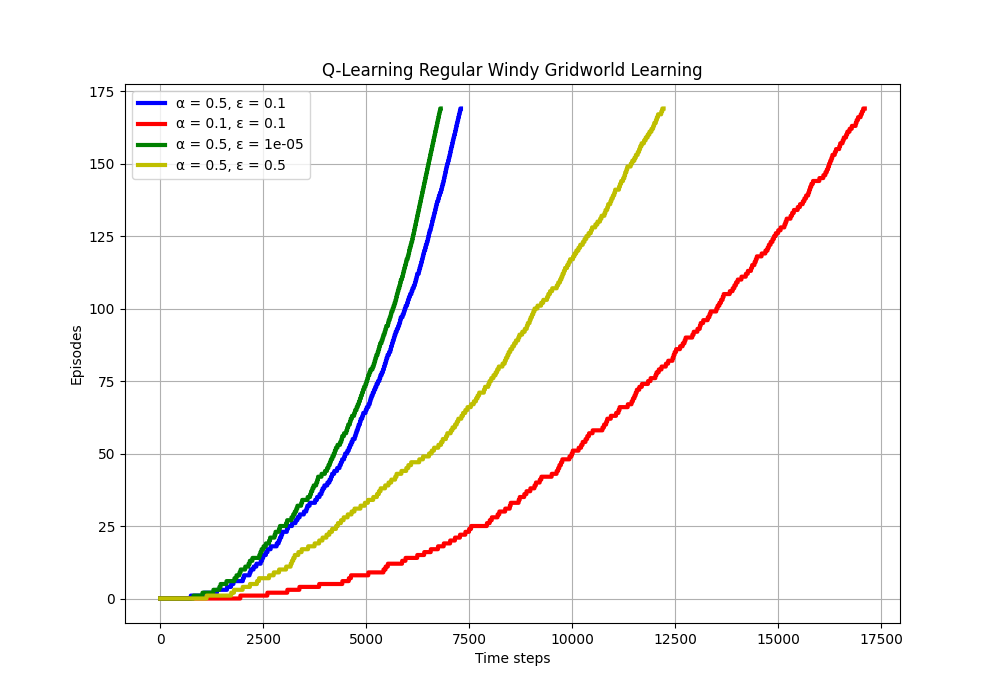
\includegraphics[width=\textwidth]{q_regular.png}
    \caption{Q-Learning}
  \end{subfigure}
  \caption{Sarsa and Q-Learning hyperparameter value comparison over 170 episodes, in normal gridworld. Values $\alpha = 0.5, \epsilon = 0.1$ performed very well, although $\alpha = 0.5, \epsilon = 1e-5$ performed slightly better for both methods. In this case, a greedier action selection strategy (selecting non-optimal actions less frequently due to smaller $\epsilon$) appears to complete episodes faster while still exploring sufficiently.}
  \label{fig:hyperparam}
\end{figure}

Figure \ref{fig:regular_example} shows example of the optimal policy learned using Sarsa and Q-Learning over 170 episodes for standard values of $\alpha = 0.5, \epsilon = 0.1$, as well as the optimal path length and average steps over the second half of all episodes. 


\begin{figure}[h!]
  \centering
  \begin{subfigure}{0.45\textwidth} 
    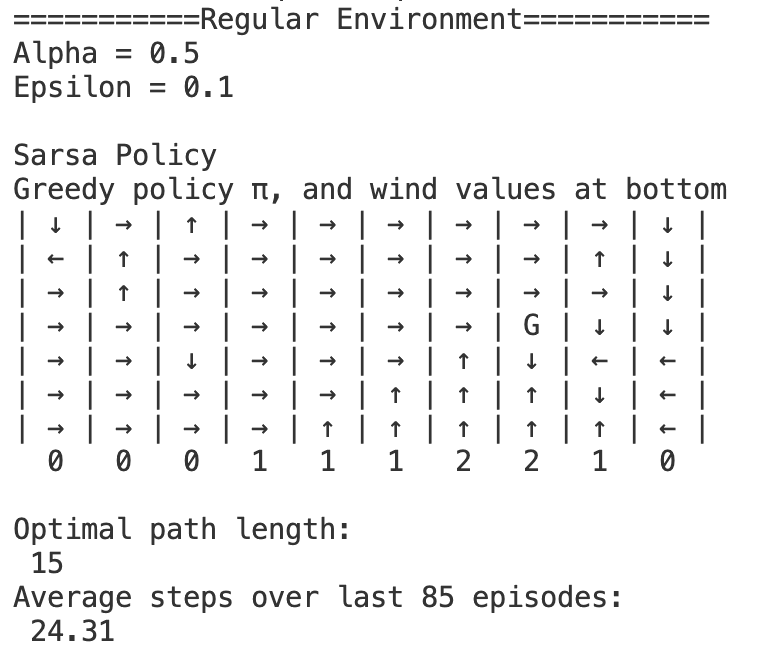
\includegraphics[width=\textwidth]{sarsa_regular_example.png}
    \caption{Sarsa}
  \end{subfigure}
  \hspace{0.05\textwidth}  
  \begin{subfigure}{0.45\textwidth}  
    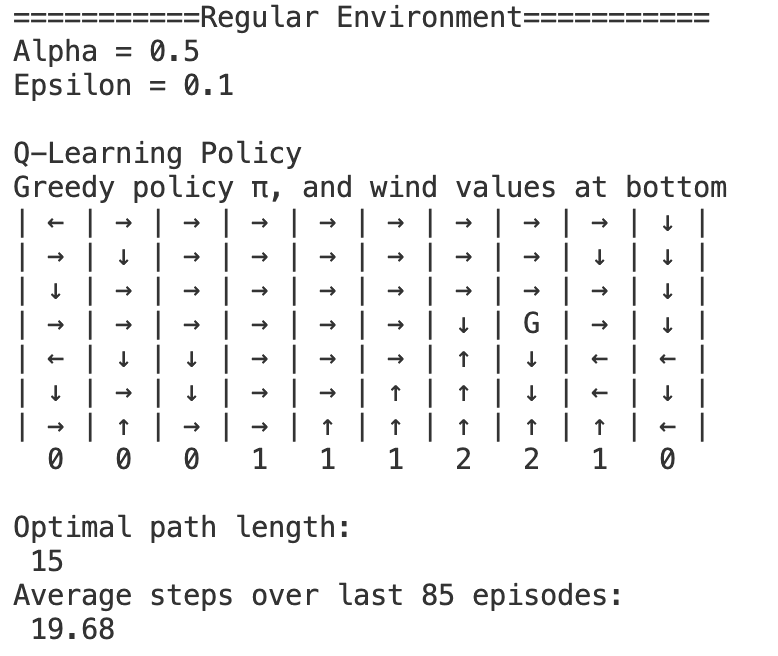
\includegraphics[width=\textwidth]{q_regular_example.png}
    \caption{Q-Learning}
  \end{subfigure}
  \caption{Sarsa and Q-Learning greedy policy and statistics, in normal gridworld. In this case, both methods found the optimal path with length 15.}
  \label{fig:regular_example}
\end{figure}

\subsection{Comparison of $Sarsa(\lambda), Q(\lambda)$}

\section{Stochastic Windy Gridworld}
Next, I investigate the modified windy gridworld, with stochastic wind and King's moves (the agent can move diagonally in all directions as well).

\begin{figure}[h!]
  \centering
  \begin{subfigure}{0.45\textwidth} 
    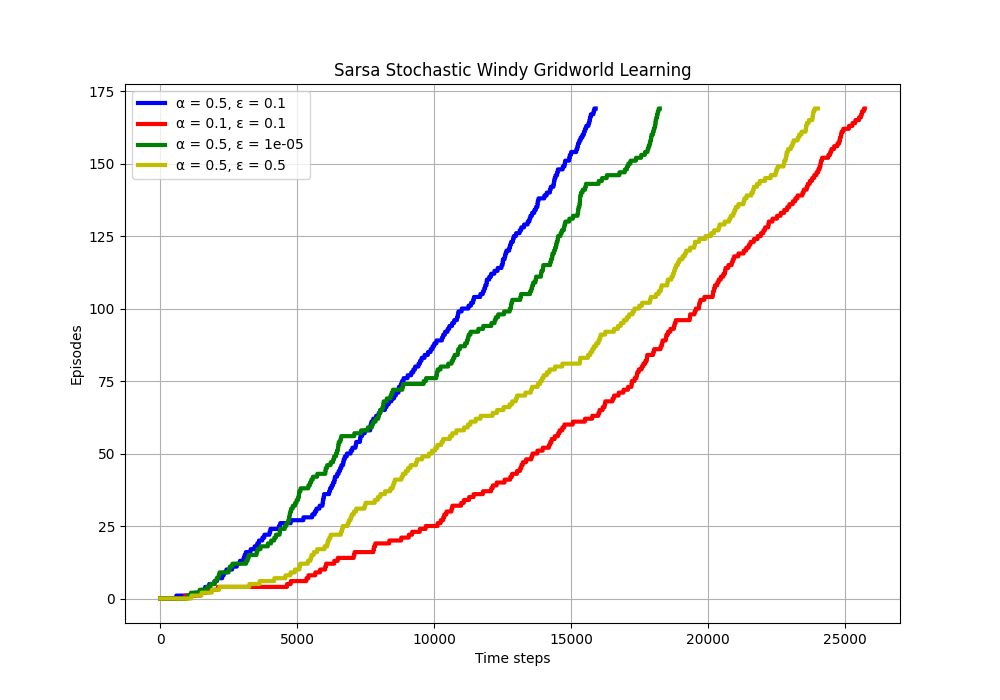
\includegraphics[width=\textwidth]{sarsa_stochastic.png}
    \caption{Sarsa}
  \end{subfigure}
  \hspace{0.05\textwidth}  
  \begin{subfigure}{0.45\textwidth}  
    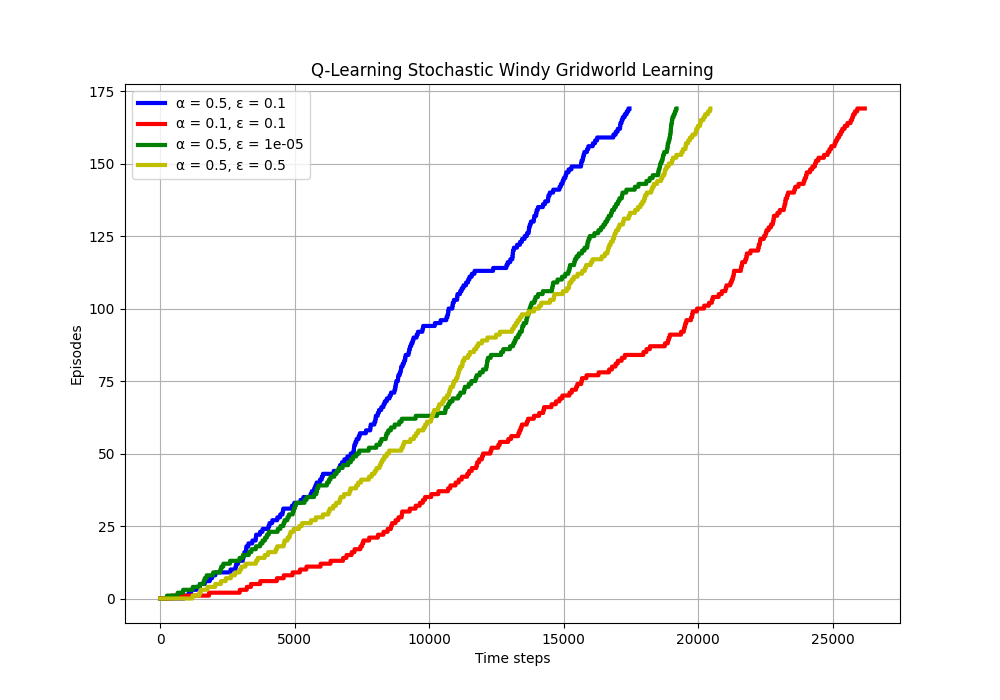
\includegraphics[width=\textwidth]{q_stochastic.png}
    \caption{Q-Learning}
  \end{subfigure}
  \caption{Sarsa and Q-Learning hyperparameter value comparison over 170 episodes, in stochastic gridworld. Standard values of $\alpha = 0.5, \epsilon = 0.1$ performed best, but learning was slower and less stable than regular gridworld, due to the larger number of action choices and the stochastic environment.}
  \label{fig:stochastic_hyperparam}
\end{figure}

\begin{figure}[h!]
  \centering
  \begin{subfigure}{0.45\textwidth} 
    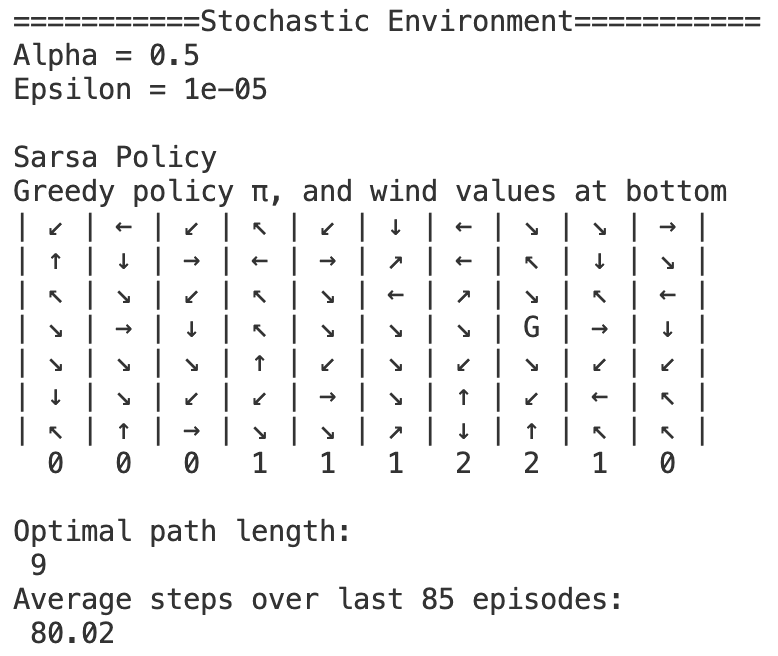
\includegraphics[width=\textwidth]{sarsa_stochastic_example.png}
    \caption{Sarsa}
  \end{subfigure}
  \hspace{0.05\textwidth}  
  \begin{subfigure}{0.45\textwidth}  
    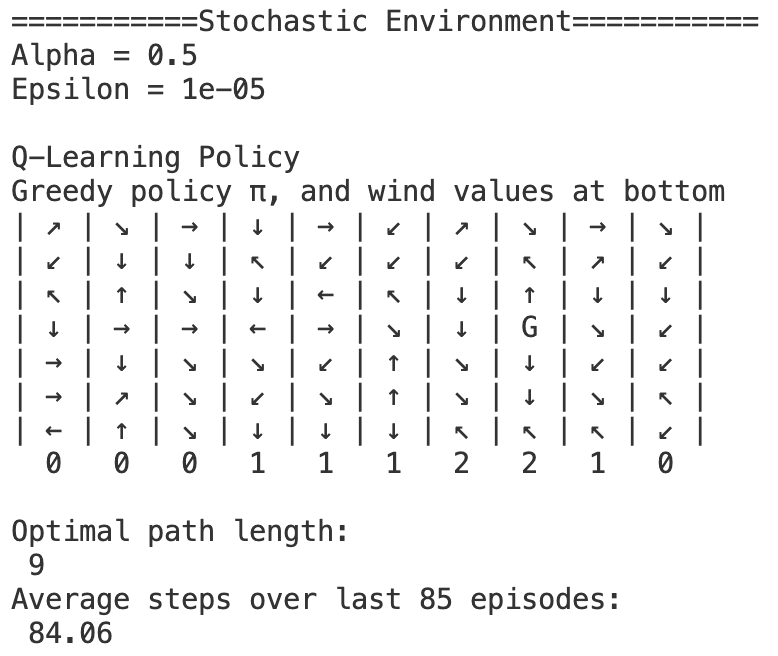
\includegraphics[width=\textwidth]{q_stochastic_example.png}
    \caption{Q-Learning}
  \end{subfigure}
  \caption{Sarsa and Q-Learning greedy policy and statistics, in stochastic gridworld. The path is shorter than regular gridworld due to diagonal movement ability.}
  \label{fig:stochastic_example}
\end{figure}

\end{document}
